% !TEX encoding = UTF-8 Unicode
% !TEX TS-program = pdflatex
% !TEX root = Relazione12.tex
% !TEX spellcheck = it-IT

\documentclass[a4paper,10pt]{article}
\usepackage[utf8]{inputenc}
\usepackage[T1]{fontenc}	
\usepackage[italian]{babel}

\usepackage{amsmath}
\usepackage{amsfonts}
\usepackage{amssymb}

\usepackage{graphicx}
\usepackage[dvipsnames]{xcolor}  %colori

\usepackage[left=2cm,right=2cm,top=2cm,bottom=2cm]{geometry}
\geometry{a4paper}
\setlength\marginparwidth{40pt}
\setlength\marginparsep{1pt}

\usepackage{verbatim}
\usepackage{lipsum}

\usepackage{booktabs}
\usepackage{subfig}
\usepackage{float}
\usepackage{wrapfig}

\usepackage[colorlinks=true, linkcolor=black, urlcolor=blue, citecolor=darkgray, filecolor=darkgray]{hyperref}   %per gli hyperlink
\usepackage[italian, sort, noabbrev, capitalise]{cleveref}
\usepackage[bottom]{footmisc}

\usepackage[cdot, thickqspace, squaren]{SIunits}

% macro
\def\code#1{\texttt{#1}}

\title{Esercitazione 12: Flip-Flop e contatori}
\author{Gruppo BL \\ Candido Alessandro, Luzio Andrea, Mazziotti Fabrizio}

\begin{document}

\maketitle

\section{Scopo e Strumentazione}
Costruire alcuni circuiti logici sequenziali, progressivamente
più complessi.

La strumentazione è quella solitamente presente sul banco di lavoro, e inoltre si è usato:
\begin{itemize}
	\item Circuiti integrati;
	\begin{itemize}
		\item \code{SN74LS00} Quad NAND Gate (x2);
		\item \code{SN74LS93} 4-bit binary counter;
		\item \code{SN74LS74} Dual D-Latch (x2);
		\item \code{SN74LS86} Quad XOR Gate;
	\end{itemize}
	\item 1 DIP Switch a 4 interuttori;
	\item 1 pulsante (doppio contatto: 1 normalmente chiuso, 1 normalmente aperto);
	\item 4 diodi LED.
\end{itemize}




\section{Flip-Flop D-Latch}

\begin{figure}[H]
	\centering
	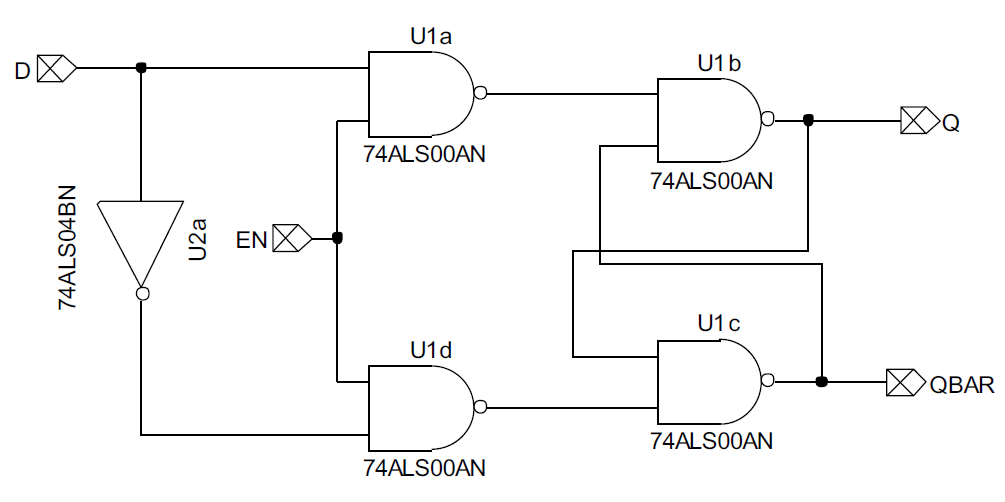
\includegraphics[width=0.7\textwidth]{../grafici/FlipFlopD.png}
	\caption{Schema del circuito del Flip-Flop di tipo D}
	\label{fig:FFD}
\end{figure}
Si è montto il circuito in \cref{fig:FFD} e si è verificato il funzionamento del circuito inviando in $D$ il segnale proveniente dal generatore di funzioni. Si è ripetuto il procedimento diverse volte, accendendo e spegnendo l'enable $E$ (controllato con uno swich) per verificare che, come previsto:\\

\begin{itemize}
\item Se l'enable è \code{HIGH} il segnale $D$ venga semplicemente ripetuto in $Q$
\item Se l'enable è \code{LOW} il segnale è stabile
\item Il valore di $Q$ (e dunque di $Q$bar) vengono conservati una volta che il dispositivo è disabilitato.
\end{itemize}

Per supportare tali verifiche sono state prese le seguenti immagini:


\begin{figure}[H]
	\centering
	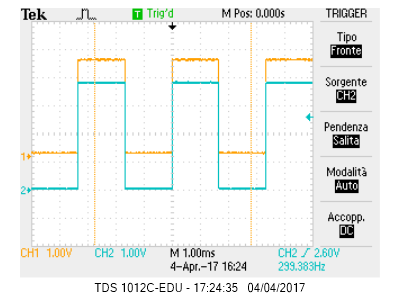
\includegraphics[width=0.7\textwidth]{../grafici/enableUp.png}
	\caption{Q segue D se l'enable è \code{HIGH}}
	\label{fig:FFD}
\end{figure}

\begin{figure}[H]
	\centering
	\includegraphics[width=0.7\textwidth]{../grafici/EnableDown0.png}
	\caption{Q congelato su \code{HIGH} mentre l'enable è \code{LOW}}
	\label{fig:FFD}
\end{figure}

\begin{figure}[H]
	\centering
	\includegraphics[width=0.7\textwidth]{../grafici/EnableDown1.png}
	\caption{Q congelato su \code{LOW} mentre l'enable è \code{LOW}}
	\label{fig:FFD}
\end{figure}

Come è mostrato nelle figure capita sia che $Q$ venga congelato nel suo valore \code{HIGH} che nel suo valore \code{LOW} in base allo stato logico dell'uscita quando l'enable viene diabilitato.\\
Dalla prima immagine è invecie palese che l'uscita della porta si limita a seguire l'ingresso se l'enable è abilitato.\\
Oltre alla mera verifica del funzionamento si è qunque misurato il ritardo fra l'ingresso e l'uscita, nella condizione %$E=$\code{HIGH}, di $V_{rit}=\unit{32\pm 2}{\Ohm}$



\section{Divisori di frequenza}

\begin{figure}[H]
	\centering
	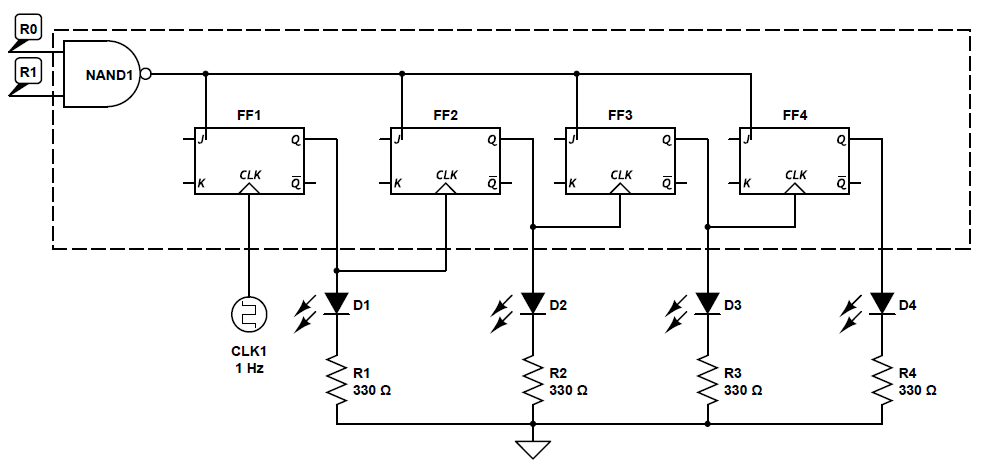
\includegraphics[width=0.9\textwidth]{../grafici/counterScheme.png}
	\caption{Schema del circuito del contatore a 4 bit}
	\label{fig:counter}
\end{figure}

\pagebreak

\section{Shift register con D-Latch}

\begin{wrapfigure}{R}{0.4\textwidth}
	\vspace{-20pt}
	\centering
	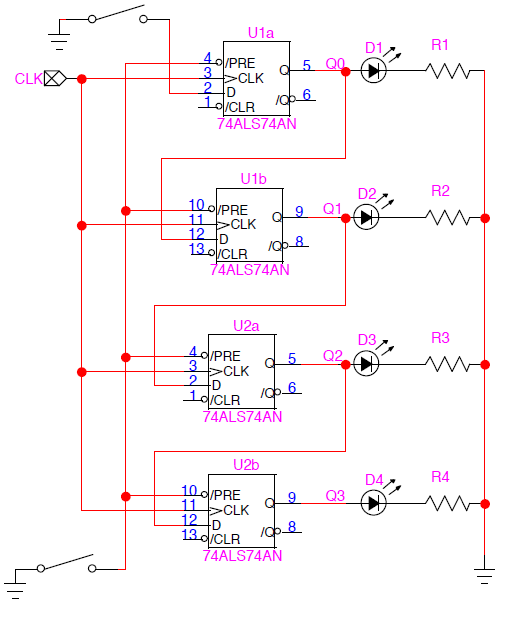
\includegraphics[width=0.4\textwidth]{../grafici/shiftreg.png}
	\vspace{-10pt}
	\caption{Schema del circuito dello shift register}
	\label{fig:shift}
	\vspace{-40pt}
\end{wrapfigure}

Si è realizzato il circuito in \cref{fig:shift}, impiegando resistenza da $\sim \unit{330}{\ohm}$ e alimentando il tutto a $\sim \unit{5}{\volt}$.

In un primo momento si è provato a non inserire alcuna resistenza di pull-up, e si verificato che in un buon numero di casi lo shift register si comportava come atteso (e.g.: tutti i bit a 0 e un singolo 1 che "viaggia", oppure la situazione reciproca, funzionavano senza inconvenienti). 
Per fare ciò si è impostato un clock a frequenza molto bassa, in modo da realizzare le configurazioni desiderate dello shift register agendo solo sull'interruttore sul DIP Switch, cioè inviando manualmente i dati al primo Flip-Flop del registro (U$1$a in \cref{fig:shift}).

Si è dunque continuato verificando lo stato delle uscite dopo aver premuto il pulsante di preset, e questo è risultato essere \code{HIGH} (LED accesi), che è quanto atteso per il comportamento dei Flip-Flop di questo tipo (si sarebbe ottenuto l'opposto se si fosse scelto di pilotare con il pulsante gli ingressi di clear).

\section{Generatore di sequenze pseudo-casuali}

\begin{wrapfigure}{L}{0.4\textwidth}
	\vspace{-5pt}
	\centering
	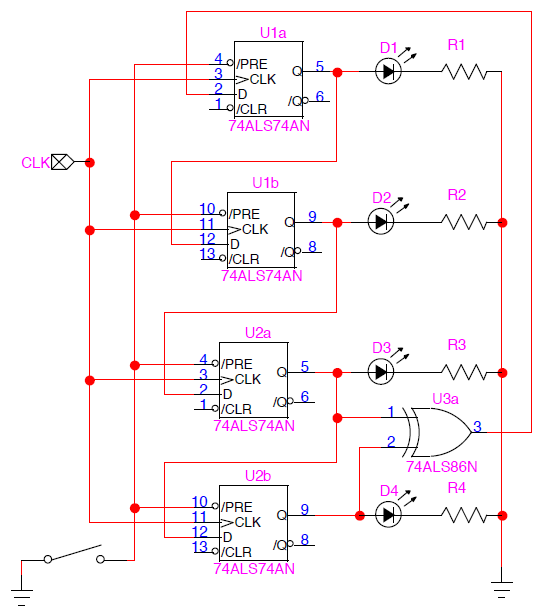
\includegraphics[width=0.4\textwidth]{../grafici/randomseq.png}
	\vspace{-5pt}
	\caption{Schema del circuito del generatore di sequenze pseudo-casuali}
	\label{fig:random}
	\vspace{-5pt}
\end{wrapfigure}

Si è aggiunto allo shift register, \cref{fig:shift}, un "tap", realizzato con uno XOR che connettesse le uscite dei due bit più significativi (U$2$a e U$2$b in \cref{fig:random}) all'ingresso del bit meno significativo (U$1$a in \cref{fig:random}), sostituendo il collegamento all'interruttore realizzato per testare lo shift register.
\newline

Si è inviato un clock a bassa frequenza e si è premuto il pulsante di preset, lasciando che il circuito evolvesse a partire dalla configurazione con tutti i LED accesi (tutte le uscite \code{HIGH}).

Si è osservato che il circuito compieva un loop di $15$ stati, evitando lo stato in cui tutti i LED siano spenti (tutte le uscite \code{LOW}), che analizzando rapidamente il circuito risulta subito essere uno stato stabile, che quindi "bloccherebbe" l'evoluzione.

\paragraph{Resistenze di pull-up}A differenza del circuito precedente in un primo momento il circuito sembrava non funzionare correttamente: il ciclo precedentemente descritto era eseguito fino allo stato 9) (vedi sotto), mentre la transizione successiva lo riportava direttamente allo stato 1) (qualitativamente si notava anche una differenza nell'accensione/spegnimento dei LED rispetto alle altre transizioni).

Si è dunque reinserito l'interruttore e si sono provate diverse configurazioni, individuando il problema nella transizione di U$2$a in poche configurazioni, si è dunque provato a inserire una resistenza di pull-up da $\sim \unit{1}{\kilo\ohm}$ tra il clear di questo Flip-Flop e Vcc. \marginpar{Confermate che era il clear?}
Questo ha infine risolto il problema, e il circuito si è comportato come atteso.

\paragraph{Ciclo pseudo-casuale} Si riportano quindi in ordine gli stati osservati nel corso del ciclo completo:

\begin{equation*}
\begin{matrix}
1)	&		&	1	&	1	&	1	&	1	\\
2)	&		&	0	&	1	&	1	&	1	\\
3)	&		&	0	&	0	&	1	&	1	\\
4)	&		&	0	&	0	&	0	&	1	\\
5)	&		&	1	&	0	&	0	&	0	\\
6)	&		&	0	&	1	&	0	&	0	\\
7)	&		&	0	&	0	&	1	&	0	\\
8)	&		&	1	&	0	&	0	&	1	\\
\end{matrix}
\qquad \qquad
\begin{matrix}
9)	&		&	1	&	1	&	0	&	0	\\
10)	&		&	0	&	1	&	1	&	0	\\
11)	&		&	1	&	0	&	1	&	1	\\
12)	&		&	0	&	1	&	0	&	1	\\
13)	&		&	1	&	0	&	1	&	0	\\
14)	&		&	1	&	1	&	0	&	1	\\
15)	&		&	1	&	1	&	1	&	0	\\
\end{matrix}
\end{equation*}

\paragraph{Altri "tap" possibili} Si è trovato in rete che qualunque scelta si faccia per la coppia che genera il "tap", si ottiene un ciclo su tutti i $15$ stati possibili\footnote{Cioè escluso quello stabile.}:
\newline
\newline
\href{https://www.slideshare.net/azadajay/prbs-generation-using-s}{https://www.slideshare.net/azadajay/prbs-generation-using-s}
\newline
\newline
Si nota che nel documento citato si fa uso di una porta XNOR, ma, a patto di scambiare lo stato iniziale da tutti \code{LOW} a tutti \code{HIGH}, è equivalente.

\end{document}